%% -*- TeX-engine: luatex; ispell-language: "russian" -*-

\documentclass[a4paper,12pt]{article}
\usepackage{subcaption}
\usepackage[left=1.5cm,right=2cm,top=1.5cm,bottom=2cm]{geometry}

\usepackage{parskip}
\setlength{\parindent}{0mm}
\setcounter{secnumdepth}{1}

\usepackage{amsmath}

\usepackage{fontspec}
\setmainfont{PT Serif}
\newfontfamily\cyrillicfont[Script=Cyrillic,Ligatures=TeX]{PT Serif}
\setsansfont{PT Sans}
\setmonofont[Ligatures=NoCommon]{PT Mono}
\defaultfontfeatures{Ligatures=TeX}

\usepackage[bold-style=ISO]{unicode-math}
\setmathfont{XITS Math}

\usepackage{microtype}

\usepackage{hyperref}

\usepackage{polyglossia}
\setmainlanguage{russian}
\setotherlanguage{english}

\usepackage{csquotes}

%% for code snippets
\usepackage{minted}
\newminted[pycon]{pycon}{fontsize=\footnotesize}
\newminted[python3]{python3}{fontsize=\footnotesize}
\newminted[bash]{bash}{fontsize=\footnotesize}
\newmintinline[pythoninline]{python3}{fontsize=\footnotesize}
\newmintinline[bashinline]{bash}{fontsize=\footnotesize}

\pagestyle{empty}


\begin{document}
\subsection*{Домашнее задание №2: <<Comic-Con и k-means>>}

\begin{tabular}{@{}lr}
  \textbf{Дедлайн 1} (20 баллов): & 10 марта, 23:59 \\
  \textbf{Дедлайн 2} (10 баллов): & 17 марта, 23:59
\end{tabular}

Домашнее задание нужно написать на Python и сдать в виде одного файла.
Правило именования файла: \texttt{name\_surname\_2.py}. Например, если
вас зовут Иван Петров, то имя файла должно быть: \texttt{ivan\_petrov\_2.py}.

\makebox[\linewidth]{\hrulefill}

На этот раз мы решили отправиться на Comic-Con. В рамках подготовки к нему нужно напечатать футболки с изображением Бэтмена и Супермена. В нашем распоряжении оказалась только одна картинка, на которой присутствуют необходимые персонажи%
\footnote{\url{https://gist.github.com/ktisha/a898e6a7a7d45b4183b0}} и принтер для печати по ткани, печатающий в 16-цветном режиме. С помощью алгоритма k-средних нужно сделать новое изображение наших героев с использованием только 16 цветов.

\paragraph{1} Каждый пиксель изображения несет информацию о своём цвете из модели RGB (цветовая модель изображения, которая состоит из трех компонентов R — red, G — green, B — blue). Значение каждой компоненты RGB может быть в пределах 0 $\dots $ 255. Это дает возможность закодировать 255*255*255 цветов.\\ 
Для работы с изображениями в Python есть библиотека-обёртка над OpenCV \footnote{\url{http://docs.opencv.org/3.0-beta/doc/py\_tutorials/py\_setup/py\_intro/py\_intro.html\#intro}}. С ее помощью выполнить задание будет проще.\\
Первым делом нам необходимо реализовать функцию, которая читает файл и преобразует его в двумерную матрицу  размерности ($M \times N	$, 3). 
Сигнатура функции следующая:
\begin{python3}
def read_image(path):
    # ...
    # подсказка: если вы используете библиотеку cv, 
    # не забудьте перевести изображение в формат rgb
    return image
\end{python3}


\paragraph{2} Следующий шаг -- реализовать функцию \pythoninline{k_means(X, n_clusters, distance_metric)}, которая принимает матрицу $X$ размерности \pythoninline{(n_samples, n_features)}, количество кластеров, на которые мы хотим разбить изображение и метрику. Результатом функции является пара из вектора размера \pythoninline{n_samples}, где в $i$-й ячейке содержится кластер, соответствующий $i$-му пикселю, и вектора размера \pythoninline{(n_clusters)} с центрами кластеров

\paragraph{3} Для оценки результата работы реализуйте две функции.\\
Первая функция \pythoninline{centroid_histogram(labels)} строит гистограмму на основе количества пикселей, приписанных каждому кластеру и возвращает ее в виде вектора.
Вторая функция \pythoninline{plot_colors(hist, centroids)} принимает построенную гистограмму и список центров кластеров и строит bar chart, показывающий относительную частоту каждого цвета. \\

\clearpage
Пример: 
\begin{figure}[htbp]
  
\includegraphics{images/barchart}   
\end{figure}

Функция может выглядеть так:\\
\begin{python3}
def plot_colors(hist, centroids):
    # инициализировать переменные bar и start_x

    for (percent, color) in zip(hist, centroids):
        # вычислить end_x
        cv2.rectangle(bar, (int(start_x), 0), (int(end_x), 50),
            color.astype("uint8").tolist(), -1)
        # обновить значение start_x

    return bar
	
\end{python3}


\paragraph{4} Последняя фунция \pythoninline{recolor(image, n_colors)} принимает изображение и количество цветов, и перекрашивает каждый пиксель изображения в тот цвет, к которому его отнес метод \pythoninline{k_means}.


\paragraph{5} Результатом работы программы должно быть изображение, в котором присутствуют только 16 цветов.


\begin{figure}[htbp]
        \centering
        \begin{subfigure}[b]{0.45\textwidth}
                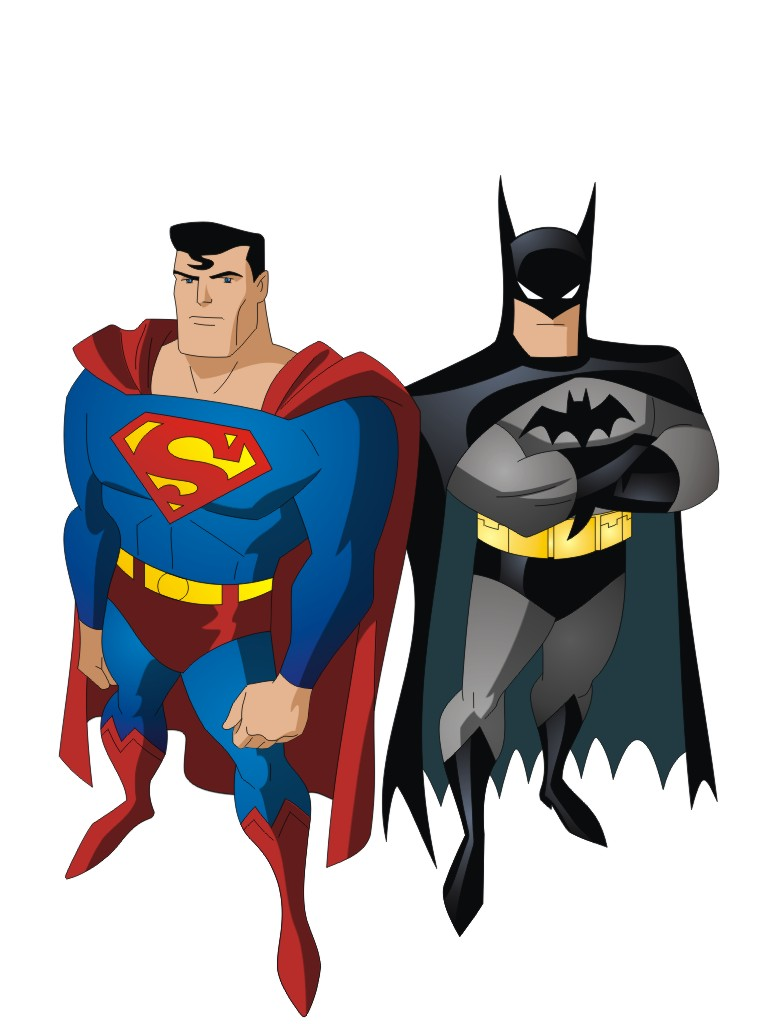
\includegraphics[width=\textwidth]{images/superman-batman}
                \caption{Исходное изображение}
        \end{subfigure}%
        ~ 
        \begin{subfigure}[b]{0.45\textwidth}
                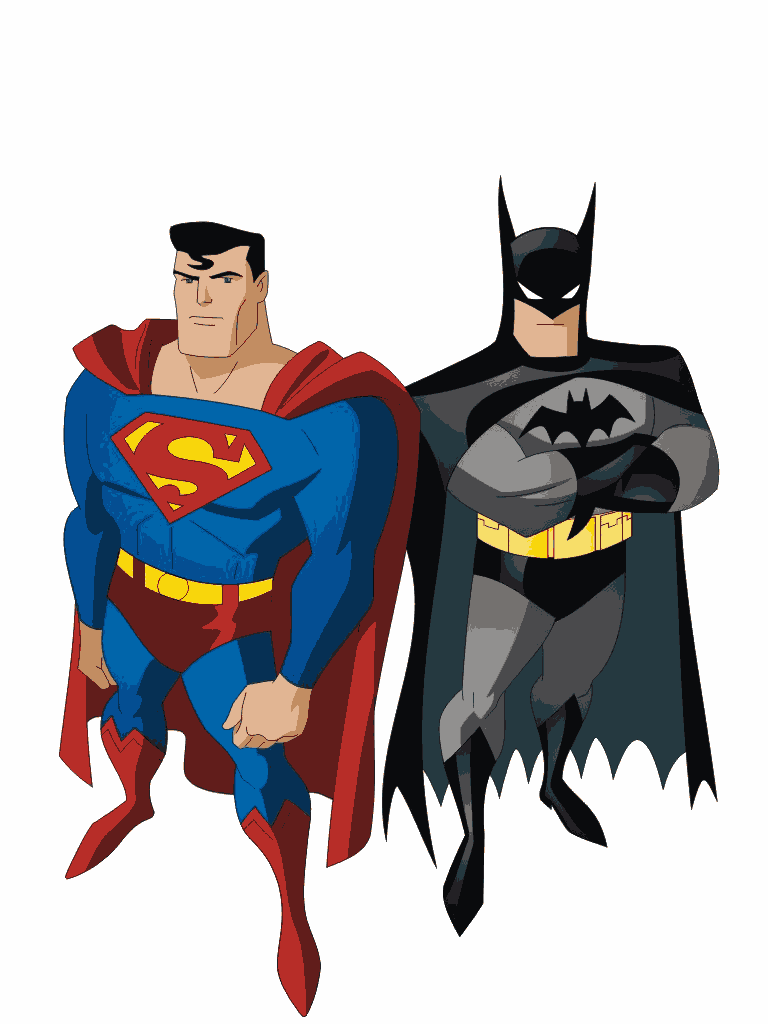
\includegraphics[width=\textwidth]{images/superman-batman-after}
                \caption{16-цветное изображение}
        \end{subfigure}
\end{figure}

\end{document}
